\documentclass[11pt,oneside]{article}
\usepackage[T1]{fontenc}
\usepackage[utf8]{inputenc}
%\DeclareUnicodeCharacter{00A0}{ }
\usepackage[adobe-utopia]{mathdesign}

\usepackage{amsmath}
\usepackage[francais]{babel}
\usepackage[dvips]{graphicx}
%\usepackage{here}
\usepackage{framed}
\usepackage[normalem]{ulem}
\usepackage{fancyhdr}
\usepackage{titlesec}
\usepackage{vmargin}

\usepackage{amsmath}
\usepackage{ifthen}
\usepackage{multirow}
\usepackage{multicol} % Portions de texte en colonnes

%\usepackage{xltxtra} % Logo XeLaTeX
%\usepackage{pst-solides3d}
\usepackage{color}
%\usepackage{colortbl}
\usepackage{titletoc} % Pour la mise en forme de la table des matières

%\usepackage[crop=off]{auto-pst-pdf}
%\usepackage{bclogo}


%\usepackage{longtable}
%\usepackage{flafter}%floatants après la référence
%\usepackage{pst-solides3d}
%\usepackage{pstricks}
%\usepackage{minitoc}
%\setcounter{minitocdepth}{4}
%\usepackage{draftcopy}% "Brouillon"
%\usepackage{floatflt}
%\usepackage{psfrag}
%\usepackage{listings} % Permet d'insérer du code de programmation
%\usepackage{lmodern}
%\usepackage[adobe-utopia,uppercase=upright,greeklowercase=upright]{mathdesign}
%\usepackage{minionpro}
%\usepackage{pifont}
%\usepackage{amssymb}
%\usepackage[francais]{varioref}

\setmarginsrb{1.5cm}{1cm}{1cm}{1.5cm}{1cm}{1cm}{1cm}{1cm}

\definecolor{gris25}{gray}{0.75}
\definecolor{bleu}{RGB}{18,33,98}
\definecolor{bleuf}{RGB}{42,94,171}
\definecolor{bleuc}{RGB}{231,239,247}
\definecolor{rougef}{RGB}{185,18,27}
\definecolor{rougec}{RGB}{255,230,231}
\definecolor{vertf}{RGB}{103,126,82}
\definecolor{vertc}{RGB}{220,255,191}
\definecolor{violetf}{RGB}{112,48,160}
\definecolor{violetc}{RGB}{230,224,236}
\definecolor{jaunec}{RGB}{220,255,191}
\usepackage[raccourcis]{FAST}
\usepackage[%
    pdftitle={Systèmes à événements discrets},
    pdfauthor={Xavier Pessoles},
    colorlinks=true,
    linkcolor=blue,
    citecolor=magenta]{hyperref}
\usepackage{schemabloc}



% \makeatletter \let\ps@plain\ps@empty \makeatother
%% DEBUT DU DOCUMENT
%% =================
\sloppy
\hyphenpenalty 10000

\newcommand{\Pointilles}[1][3]{%
\multido{}{#1}{\makebox[\linewidth]{\dotfill}\\[\parskip]
}}


\colorlet{shadecolor}{orange!15}

\newtheorem{theorem}{Theorem}


\begin{document}


\newboolean{prof}
\setboolean{prof}{true}
%------------- En tetes et Pieds de Pages ------------
\pagestyle{fancy}
\renewcommand{\headrulewidth}{0pt}

\fancyhead{}
\fancyhead[L]{%
\noindent\noindent\begin{minipage}[c]{2.6cm}
%Lycée Rouvière PTSI

\includegraphics[width=2cm]{png/logo_ptsi.png}%
\end{minipage}
}

\fancyhead[C]{\rule{12cm}{.5pt}}

\fancyhead[R]{%
\noindent\begin{minipage}[c]{3cm}
\begin{flushright}
\footnotesize{\textit{\textsf{Sciences Industrielles\\ pour l'Ingénieur}}}%
\end{flushright}
\end{minipage}
}

\renewcommand{\footrulewidth}{0.2pt}

\fancyfoot[C]{\footnotesize{\bfseries \thepage}}
\fancyfoot[L]{\footnotesize{2012 -- 2013} \\ X. \textsc{Pessoles}}
\ifthenelse{\boolean{prof}}{%
\fancyfoot[R]{\footnotesize{TD -- CI 8 : SED -- P}}
}{%
\fancyfoot[R]{\footnotesize{TD -- CI 8 : SED}}
}



\begin{center}
 \huge\textsc{CI 8 -- SED -- Systèmes à événements discrets}

 \large\textsc{Commande et comportement des systèmes combinatoires et séquentiels}
\end{center}

\begin{center}
 \LARGE\textsc{Chapitre 1 -- Étude des systèmes combinatoires}
\end{center}


\vspace{.5cm}
\begin{flushright}
\textit{D'après ressources de Florestan Mathurin}
\end{flushright}
%\begin{center}
%\begin{tabular}{cccc}
%\includegraphics[height=2.5cm]{png/acier} &
%\includegraphics[height=2.5cm]{png/bois} &
%\includegraphics[height=2.5cm]{png/composite} &
%\includegraphics[height=2.5cm]{png/verre}\\
%\textit{Acier \cite{acier}} & 
%\textit{Bois} & 
%\textit{Fibre de carbone \cite{composite}} & 
%\textit{Verre \cite{verre}} \\
%\end{tabular}
%\end{center}


\section*{Exercice 1 -- Escalier mécanique avec contrôle d'accès}

\begin{minipage}[c]{.45\linewidth}
Afin d'assurer la sécurité et de contrôler le nombre de personnes qui rentrent dans un ambassade, on oblige ces personnes à emprunter un escalier mécanique avec contrôle d'accès qui mène à l'étage où se situent les bureaux.

On s'intéresse au fonctionnement logique du système dont on donne le schéma de principe ainsi qu'un extrait du cahier des charges fonctionnel.


\end{minipage}
\hfill
\begin{minipage}[c]{.45\linewidth}
\begin{center}
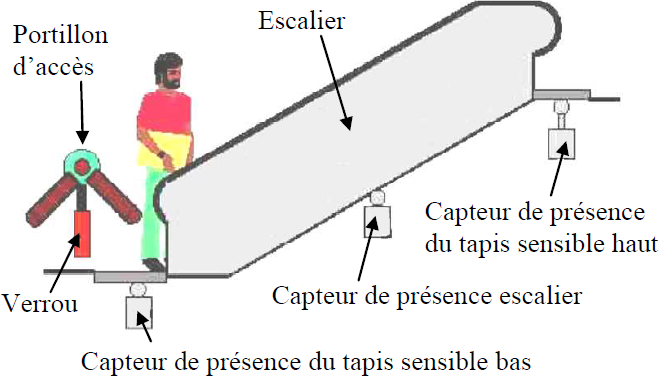
\includegraphics[width=.9\textwidth]{png/fig1}
\end{center}
\end{minipage}

\begin{center}
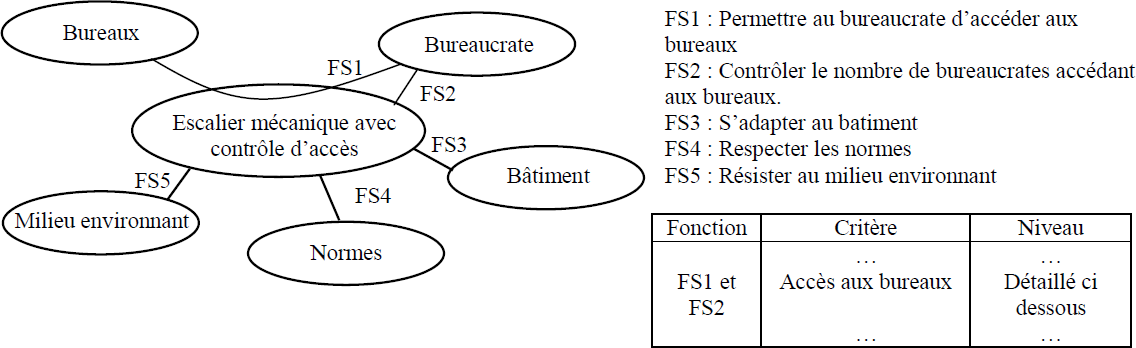
\includegraphics[width=.9\textwidth]{png/fig2}
\end{center}

\subsubsection*{Extrait du cahier des charges}
\begin{itemize}
\item Lorsqu'une personne franchi le portillon, elle pose un pied sur le tapis sensible bas ($T_b$) placé en bas de l'escalier. Aussitôt l'escalier se met en marche ($M$).
\item Dès que la personne pose un pied sur l'escalier, tout en gardant l'autre sur le tapis sensible, sa présence est détectée par un capteur de présence ($c$). Dès que ce capteur ($c$) est activé, un verrou ($V$) bloque le portillon et l'escalier continue de marcher ($M$).
\item Tout le temps que la personne reste dans l'escalier, le verrou ($V$) reste activé et l'escalier continue de marcher ($M$).
\item Dès que la personne arrive en haut de l'escalier, elle pose le pied sur le tapis sensible haut ($T_h$) mais il faut qu'il quitte l'escalier ($c$) pour que celui-ci s'arrête de marcher. Le verrou ($V$) reste actif. 
\item Lorsque la personne quitte le tapis sensible haut ($T_h$), le verrou ($V$) est désactivé. 
\item Pour tout cas indésirable, toutes les actions doivent être désactivées.
\end{itemize}

On considère que $M=1$ quand l'escalier est en marche et que $V=1$ quand le verrou est activé. 

\paragraph{}
\textit{Donner le schéma des entrées -- sorties du système.}

\paragraph{}
\textit{Construire la table de vérité permettant de décrire le fonctionnement du système.}

\paragraph{}
\textit{En déduire les équations logiques simplifiées du système.}

\paragraph{}
\textit{Construire les logigrammes permettant de décrire le fonctionnement du système.}


\section*{Coffre fort de banque}

\setcounter{paragraph}{0}

\begin{minipage}[c]{.45\linewidth}

On s'intéresse à un coffre fort de banque dont on donne le principe de fonctionnement ainsi qu'un extrait de cahier des charges ci-dessous.

\end{minipage}
\hfill
\begin{minipage}[c]{.45\linewidth}
\begin{center}
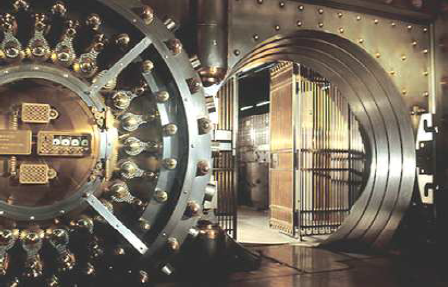
\includegraphics[width=.9\textwidth]{png/fig3}
\end{center}
\end{minipage}

\begin{center}
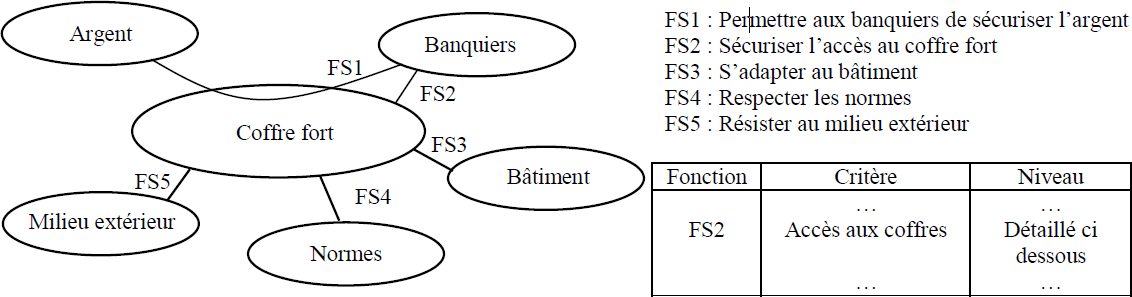
\includegraphics[width=.9\textwidth]{png/fig4}
\end{center}

\subsection*{Extrait du cahier des charges}
\begin{itemize}
\item Seuls 4 responsables (notés $A$, $B$, $C$ et $D$) qui possèdent un ensemble code d'accès + clef à serrure peuvent avoir accès au coffre. Le responsable $A$ possède l'ensemble code d'accès et une clef notée $a$. Le responsable $B$ possède l'ensemble code d'accès et une clef notée $b$. Le responsable $C$ possède l'ensemble code d'accès et une clef notée $c$. Le responsable $D$ possède l'ensemble code d'accès et une clef notée $d$.
\item Le responsable $A$ ne peut ouvrir le coffre qu'avec le responsable $B$ ou $C$.
\item Les responsables $B$, $C$ et $D$ ne peuvent ouvrir le coffre qu'en présence d'au moins deux des autres responsables.
\end{itemize}

\paragraph{}
\textit{Construire la table de vérité contenant les entrées $a$, $b$, $c$ et $d$ ainsi que la sortie $S$ ($S=1$ : coffre ouvert $S=0$ coffre fermé) permettant de décrire le fonctionnement du système.}

\paragraph{}
\textit{Donner l'équation logique non simplifiée du système du type $S=f(a,b,c,d)$.}

\paragraph{}
\textit{Simplifier cette équation à l'aide de l'algèbre de Boole.}

\paragraph{}
\textit{Simplifier l'équation logique du système obtenue avant simplification en utilisant la table de Karnaugh.}

\paragraph{}
\textit{Établir le logigramme relatif à la sortie $S$.}

\paragraph{}
\textit{Établir l'expression de $S$ qui permettra de réaliser un logigramme en n'utilisant que des portes NAND.}


\section*{Exercice 3 -- Feux de carrefour}
On s'intéresse à une intersection entre une route principale et une route secondaire dont on donne le modèle ainsi qu'un extrait du cahier des charges fonctionnel.

\setcounter{paragraph}{0}


\begin{center}
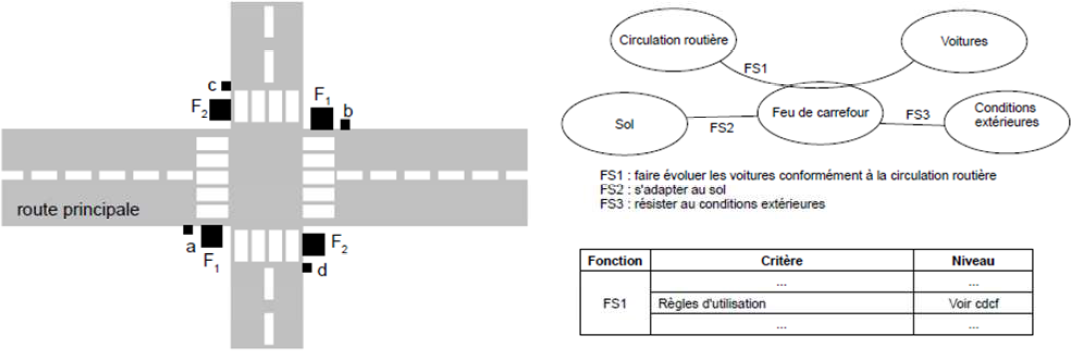
\includegraphics[width=.9\textwidth]{png/fig5}
\end{center}

Des capteurs de présence de voitures sont placés le long des voies : $a$ et $b$ pour la route principale, $c$ et $d$ pour la route secondaire. Les sorties de ces capteurs sont à A en présence de voitures. 

Le cahier des charges fonctionnel de la fonction FS1 est le suivant : 
\begin{itemize}
\item le feu $F_1$ est vert quand il y a des voitures en $a$ et $b$ en même temps;
\item le feu $F_1$ est vert quand simultanément il y a des voitures en $a$ ou $b$ et qu'il n'y a pas en $c$ ou pas en $d$;
\item le feu $F_2$ est vert quand il y a des voitures en $c$ et $d$ et qu'il n'y en a pas en $a$ ou en $b$;
\item le feu $F_2$ est vert quand il y a des voitures en $c$ et $d$ et qu'il n'y en a ni en $a$ ni en $b$;
\item le feu $F_1$ est vert quand il n'y a pas de voiture du tout.
\end{itemize}

Un feu est à 1 lorsqu'il est vert.

\paragraph{}
\textit{Déterminer l'expression de $F_1$ est de $F_2$ en sommant les conditions logiques exprimées dans les 5 points du cahier des charges.}

\paragraph{}
\textit{Réaliser les tableaux de Karnaugh de $F_1$ et $F_2$.}

\paragraph{}
\textit{Simplifier les expressions de $F_1$ et $F_2$ par les tableaux de Karnaugh.}

\paragraph{}
\textit{Tracer les organigrammes de $F_1$ et $F_2$ correspondant aux expressions obtenues. }

\paragraph{}
\textit{Déterminer par le calcul la valeur de $F_1$ ou $F_2$ (OU exclusif) et $F_1$ et $F_2$. Interpréter le résultat obtenu.}

\end{document}